\section{Conclusion}



\subsection{Benchmarking}

The Flying Squid  benchmarking infrastructure involves using ApacheBench to time file downloads through ATS with caching turned on running on an AWS EC2 instance. We hosted test files of specific sizes on our public Github organization repository.

\begin{figure}[H] \centering
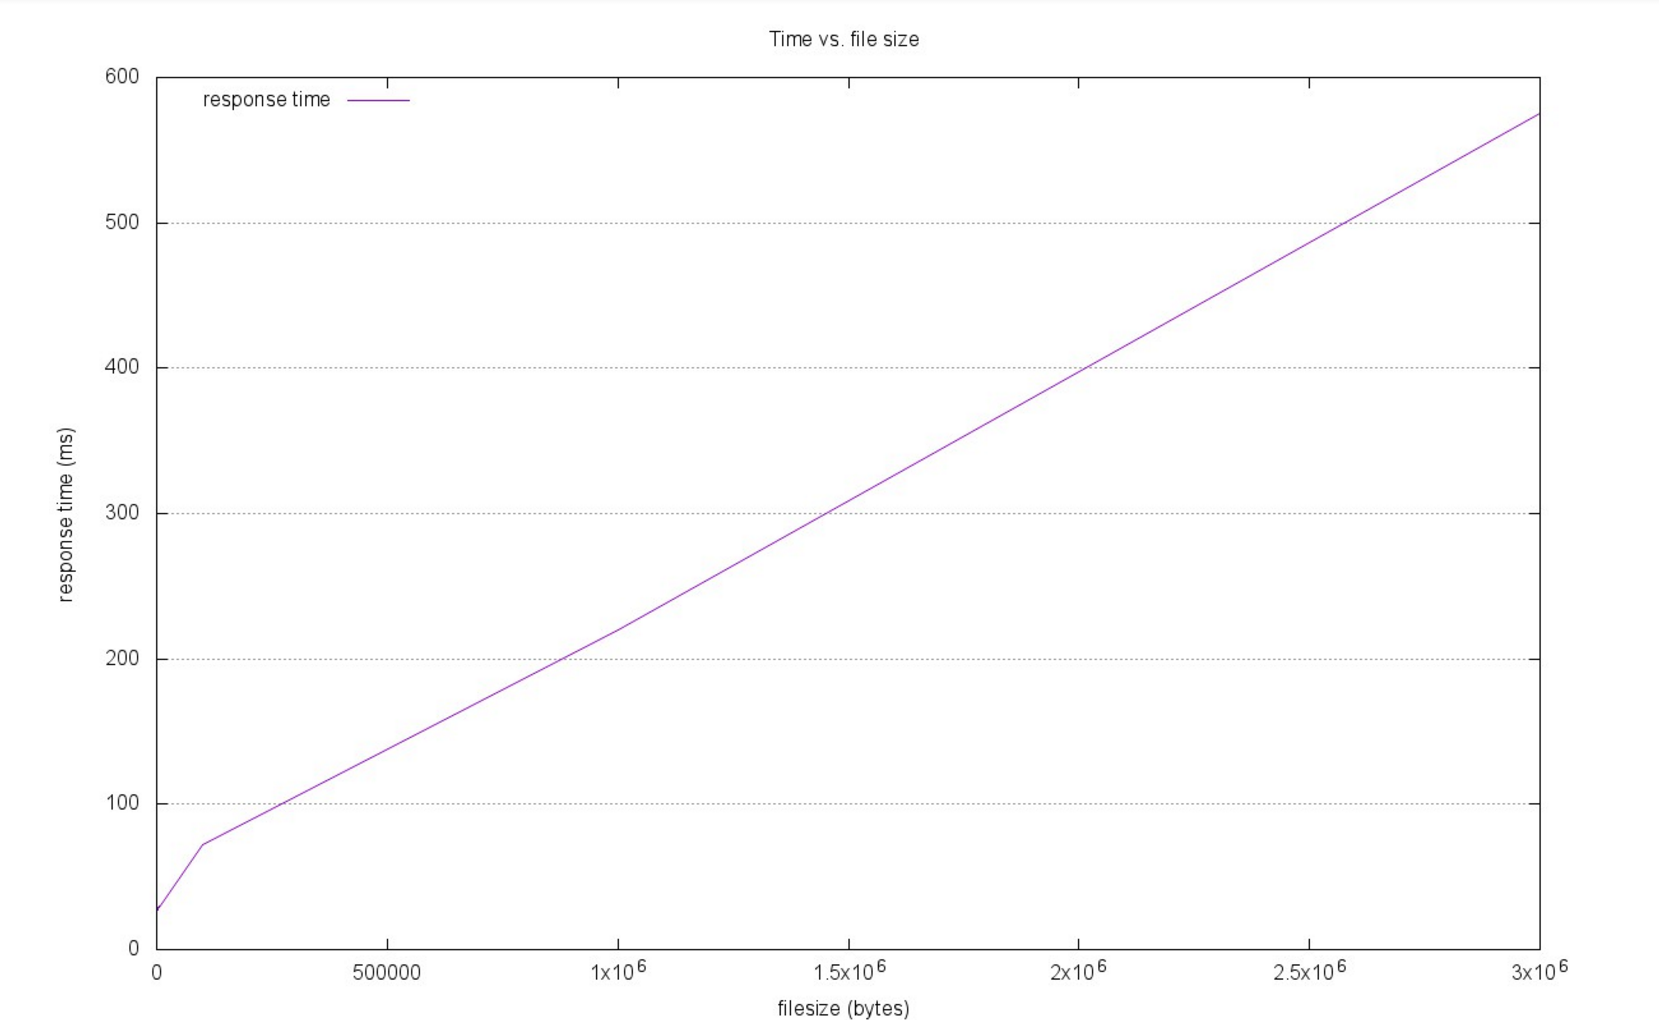
\includegraphics[width=12cm]{Benchmarking1}
\caption{Initial Benchmarks: File size vs mean service time while using standard ATS}
\end{figure}


\subsection{Further Work}

A lot of work needs to be done to make Flying Squid a production level proxy system. The proxy is only as strong as its weakest link. The integration of cloud caches, ATS and fingerprinting systems could be further streamlined. Better integration would involve more robust browser-side clients, and the elimination of redundant actions within ATS. Value based caching could be made more flexible, with adjustable block sizes and less persistent TCP connections. More benchmark and bandwidth analysis could help better understand the strengths and weaknesses of Flying Squid. Eventually, this analysis would provide grounds for interesting research.

To accurately measure the effectiveness and relevance of Flying Squid, we must investigate several use cases for our proxy server. We must leverage these use cases to show, with measurable benchmarks, that Flying Squid is indeed an improvement on the proxy status quo. First, there is the use case of a proxy network with multiple nodes to maximize personalized caching for more than just an individual. The custom caching could cater to a corporation, non-profit organization, as well as universities like Tufts. 
Many countries in the world have extremely limited bandwidth. We must account for these use cases, as these countries’ population constitute a significant part of the world’s internet users. In effect, Flying Squid will deliver content to these users at speeds faster than the speed that is currently available.


\subsection{Open Source}

We have been working with an open source fork of ATS hosted in our GitHub organization. The modifications we have made to ATS will hopefully be proposed as pull requests we can make to the main project. Several of our contributions have been placed directly in the ATS codebase. Thus, all modifications are open source contributions that we hope to be approved as part of the main Traffic Server codebase. Our GitHub repository can be found at \url{https://github.com/FlyingSquid/}.